\section{Continuous Integration}

\begin{figure}[h]
	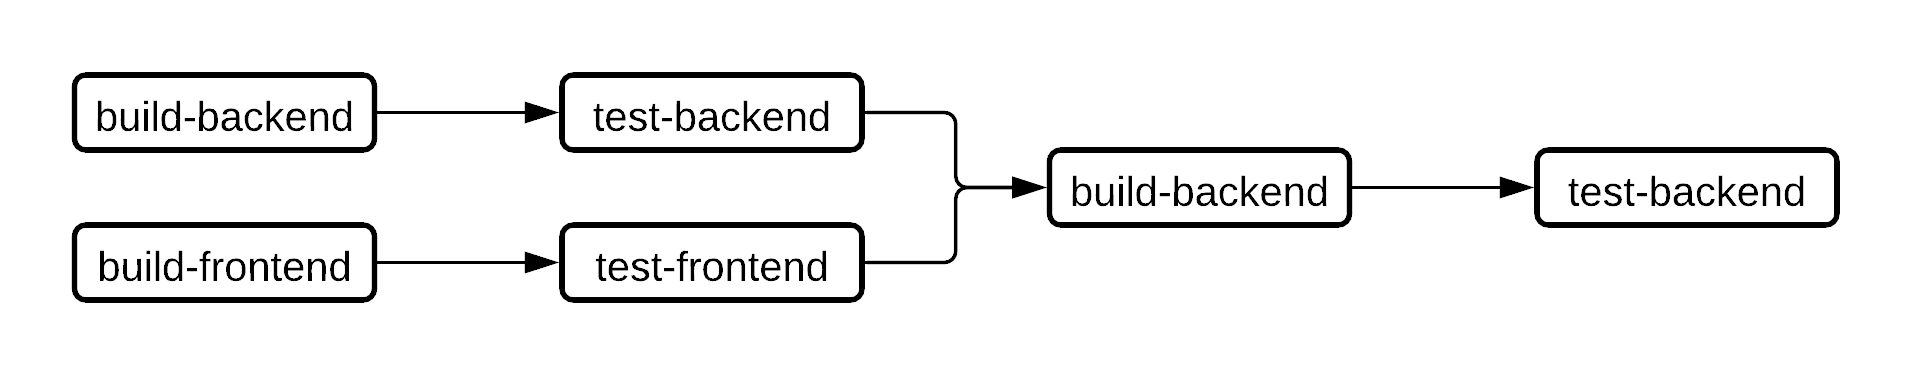
\includegraphics[width=\textwidth]{ci_diagram}
  \caption{Simple flow diagram of the continuous integration pipeline}
	\centering

\end{figure}

\subsection{Setup}
Github offers with Github Actions a service for the easy setup of continuous integration pipelines. It makes heavy use of modern technologies like virtualization and containerization. Since the repoistory for \parkview{} is hosted on Github, Github Actions is used for continuos integration. While the running of basic build and unit tests and the generation of test reports is quite trivial, the integration tests are more complex in their setup and functionality.

All integration tests are written in Python 3 and use Selenium as a web testing framework. Selenium allows us to interact with any webpage and can be used to automate a list of steps to fully test the functionality of the system. Any test cases that have to use the API offered by the backend alone make use of the requests\footnote{https://github.com/psf/requests} library for Python. It also uses the docker bindings\footnote{https://github.com/docker/docker-py} for Python for building, starting and stopping containers for the frontend and backend, since every test scenario should be run from the same starting point. Therefore every test consists of a setup and a run phase. In the setup phase any necessary actions before the actual test run take place, such as loading data into the database. The actual test run throws an exception if it fails.

\subsection{Test Run}
On startup the integration test suite builds container images for both the frontend and the backend. The backend is ran with an embedded PostgreSQL database, since it should be cleared with each restart anyway. Before each specific test run it restarts both containers to get the same conditions for every run. It then waits a configured amount of time to give the containers enough time to properly start up. Then it proceeds with the setup phase for each test, following with the run phase. It then proceeds to the next test scenario.

\subsection{Continuous Deployment}
To offer users a way to test new features and collect feedback from them we set up a small webserver. We use continuous deployment to keep that instance constantly up to date and catch bugs and possible enhancements early. The keys to that are the container images that get build by the continuous integration pipeline. After the container images are built the webserver gets notified. It then pulls the new images and and restarts the services.
